\documentclass[fontsize=12]{article}

\pagestyle{empty}

\usepackage{amsmath}
\usepackage{amsfonts}
\usepackage{amssymb}
\usepackage{rotating}
\usepackage{enumerate}
\usepackage[normalem]{ulem}
\usepackage{listings}
\usepackage[dvipsnames]{xcolor} %allows use of color
\usepackage{physics}
\usepackage{hyperref}
\usepackage{graphicx}
%\usepackage{color}
%\usepackage{listings}
\newcommand{\kB}{k_{\mathrm{B}}}
\newcommand{\kT}{\kB T}


\newcommand{\vek}[1]{\boldsymbol{#1}}          % vector symbol
\newcommand{\dif}{\mathrm{d}}                  % the d in integrals
\newcommand{\me}{\mathrm{e}}                   % Euler's e
\newcommand{\vekprod}{\! \cdot \!}
\newcommand{\eexp}[1]{\me^{\displaystyle #1}}
\newcommand{\eeexp}[1]{\me^{#1}}
\newcommand{\eeeexp}[1]{\exp \left( #1 \right)}
\newcommand{\mean}[1]{\left<#1\right>}
\newcommand{\orderof}[1]{\mathcal{O}\left(#1\right)}
\def\Real{\hbox{I\kern-.1667em\hbox{R}}}
\newcommand{\ffrac}[2]{\frac{\displaystyle #1}{\displaystyle #2}}
\renewcommand{\Re}{\operatorname{Re}}
\renewcommand{\Im}{\operatorname{Im}}
\newcommand{\dt}{\delta t}
\newcommand{\tdt}{t + \delta t}

\newcommand{\half}{\mbox{$\frac{1}{2}$}}
\newcommand{\Phat}{\mbox{$\hat P$}}
\newcommand{\Ahat}{\mbox{$\hat A$}}
\newcommand{\ekin}{\hat{E}_{kin}} 
\newcommand{\cx}{$\cos{\xi}$}
\newcommand{\sx}{$\sin{\xi}$}
\newcommand{\csx}{$\cos^2{\xi}$}
\newcommand{\ssx}{$\sin^2{\xi}$}
\newcommand{\myx}{\ensuremath{\Delta\omega t}}
\newcommand{\hmyx}{\ensuremath{\frac{\Delta\omega t}{2}}}
\definecolor{MyGreen}{RGB}{27, 94, 20}
\newcommand*{\soln}[1]{\color{MyGreen}{{#1}}\color{black}}
\newcommand*{\solution}{\soln{Solution}}


\setlength{\oddsidemargin}{0.25cm}
\setlength{\textwidth}{6in}
\setlength{\topmargin}{0in}
\setlength{\headsep}{0in}
\setlength{\textheight}{8.9in}

\newcounter{problemcounter}  
\newenvironment{problemlist}
 {\begin{list}{\textbf{Problem \arabic{problemcounter}.}~}{\usecounter{problemcounter} \labelsep=0em \labelwidth=0em \leftmargin=0em \itemindent=0em}}
 {\end{list}}


\begin{document}
\begin{center}
\textbf{Homework Set 2} \\
Chemistry 553, Spring 2021 \\
Instructor: Lutz Maibaum \\
\vspace{1em}
\textbf{Due Friday, April 16th}
\end{center}

%\lstset{frame=shadowbox, rulesepcolor=\color{blue}}
%\lstinputlisting{/Users/lutz/c/python/ljmd/ljmd.py}

\begin{problemlist}

\item 
In this problem we consider a system of $N$ indistinguishable atoms confined to a volume $V$ at a temperature $T$.
\begin{enumerate}[(a)~]
\item Show that the canonical partition function 
\begin{equation*}
Q = \ffrac{1}{N! h^{3N}} \int \dif \vek{r}^N \dif \vek{p}^N \eexp{-\left(\hat{U}(\vek{r}^N) + \hat{E}_{\mathrm{kin}}(\vek{p}^N)\right)/\kT} 
\end{equation*}
can be written as
\begin{equation*}
Q = \ffrac{1}{N! \Lambda^{3N}} Z 
\end{equation*}
where
\begin{equation*}
Z = \int \dif \vek{r}^N  \eexp{-\hat{U}(\vek{r}^N)/\kT} 
\end{equation*}
is called the configuration integral. What is $\Lambda$?
\soln{
\begin{align*}
	Q &= \frac{1}{N!h^{3N}}\int\,d{r^N}\,d{p^N}\eexp{-\left(\hat{U}(r^N) + \ekin(p^N)\right)/\kT}\\
	&= \frac{1}{N!h^{3N}} \int\,d{r^N}\eexp{-\hat{U}(r^N)/\kT}\int \,d{p^N}\eexp{\ekin{p^N}/\kT}\\
	&= \frac{Z}{N!h^{3N}}\int \,d{p^N}\eexp{\ekin{p^N}/\kT}
\end{align*}
I am not sure how this next step works. I found the result of this integral from the following website (see eq. 4):
\href{https://chem.libretexts.org/Bookshelves/Physical_and_Theoretical_Chemistry_Textbook_Maps/Supplemental_Modules_(Physical_and_Theoretical_Chemistry)/Statistical_Mechanics/Boltzmann_Average/Ideal_gas_partition_function}{Libretext: Ideal Gas Partition Function}\\
after solving the integral, set everythign equal to the other form of Q, cancel like terms, and solve for $\Lambda$
\begin{align*}
	&= \frac{Z}{N!h^{3N}}\left(2\pi m\kT\right)^{3N/2} = \frac{1}{N!\Lambda^{3N}}Z\\
	&= \left(\frac{\sqrt{2\pi m\kT}}{h}\right)^{3N} = \Lambda^{-3N}\\
	&= \left(\frac{\sqrt{2\pi m\kT}}{h}\right)^{-1} = \Lambda\\
	\Lambda &= \sqrt{\frac{h^2}{2\pi m\kT}}
\end{align*}
}

\item The ideal gas is a hypothetical system in which the atoms do not interact (i.e., the potential energy $U$ is zero for all configurations), but somehow the system can still equilibrate. Calculate the configuration integral $Z$, the partition function $Q$, the free energy $F$, and the pressure $p = - \partial F / \partial V$ of an ideal gas.\\
\soln{
We can start with the re-written form of the canonical partition function, then use the same integral evaluation as part (a):
\begin{align*}
	Q &= \frac{1}{N!h^{3N}} \int\,d{r^N}\eexp{-\hat{U}(r^N)/\kT}\int \,d{p^N}\eexp{\ekin{p^N}/\kT}\\
	&= \frac{1}{N!h^{3N}}\left(2\pi m\kT\right)^{3N/2}\int\,d{r^N}\eexp{-\hat{U}(r^N)/\kT}\\
	&= \frac{1}{N!h^{3N}}\left(2\pi m\kT\right)^{3N/2}\int\,d{r^N}\eexp{0}\\
	&= \frac{V^N}{N!h^{3N}}\left(2\pi m\kT\right)^{3N/2}\\
	&= \frac{V^N}{N!}\left(\frac{\sqrt{2\pi m\kT}}{h}\right)^{3N} = \frac{V^N}{N!\Lambda^{3N}} = \frac{1}{N!}\left(\frac{V}{\Lambda^3}\right)^N\\
	Z &= V^N\\
	F &= -\kT\ln{Q}\\
	&= -\kT\ln{\frac{1}{N!}\left(\frac{V}{\Lambda^3}\right)^N}\\
	&= -\kT\left(\ln{1}-\ln{N!} + N\ln{\frac{V}{\Lambda^3}}\right)\\
	&= -\kT\left(-N\ln{N}+N+N\ln{\frac{V}{\Lambda^3}}\right)\\
	&= -\kT N\left(-\ln{N}+1+\ln{\frac{V}{\Lambda^3}}\right)\\
	&= -\kT N\ln{\frac{Ve}{\Lambda^3N}}\\
	p &= -\pdv{F}{V} = -\pdv{}{V}\left(-\kT N\ln{V} + -\kT N\ln{\frac{e}{\Lambda^3N}}\right)\\
	&= \frac{\kT N}{V}
\end{align*}
}
\item Show that the free energy $F = -\kT \ln Q$ of an interacting system can be split into two contributions,
\begin{equation*}
F = F^{\mathrm{id}} + F^{\mathrm{ex}} ,
\end{equation*}
where $F^{\mathrm{id}}$ is the free energy of an ideal gas with same values of N, V, and T, and $F^{\mathrm{ex}}$ is called the excess free energy that is determined by the interactions between atoms. How is  $F^{\mathrm{ex}}$ related to the configurational integral $Z$? 
\soln{
\begin{align*}
	F &= -\kT\ln{Q}\\
	&= -\kT\ln{\ffrac{Z}{N! \Lambda^{3N}}}\\
	&= -\kT\left[\ln{Z}-\ln{N!}-\ln{\Lambda^{3N}}\right]\\
	&= -\kT\left[\ln{Z} -N\ln{N} + N-N\ln{\Lambda^3}\right]\\
	&=-\kT\ln{Z} - \kT N\left[-\ln{N} + 1 - \ln{\Lambda^3}\right]\\
	&=-\kT\ln{Z} - \kT N\left[\ln{\frac{e}{N\Lambda^3}}-\ln{V} + \ln{V}\right]\\
	&=-\kT\ln{Z} - \kT N\left[\ln{\frac{Ve}{N\Lambda^3}}-\ln{V}\right]\\
	&=-\kT N\ln{\frac{Ve}{N\Lambda^3}}-\kT\ln{Z} + \kT N\ln{V}\\
	&=-\kT N\ln{\frac{Ve}{N\Lambda^3}}-\kT\ln{\frac{Z}{V^N}}\\
	&= F^{id} + F^{ex}
\end{align*}
}
\end{enumerate}

\item Consider a system of $N$ atoms that interact through a pairwise additive and isotropic pair potential:
\begin{equation*}
U (\vek{r}^N) = \sum_{1 \leq i < j \leq N} u(\abs{\vek{r}_i - \vek{r}_j})
\end{equation*}
\begin{enumerate}[(a)~]
\item Calculate the force acting on atom $i$, which is given by the negative of the derivative of the potential energy with respect to the position of atom $i$:
\begin{eqnarray}
\vek{F}_i = - \nabla_i U
\end{eqnarray}
Show that the force can be expressed as
\begin{equation*}
\vek{F}_i = \sum_{j \neq i} f(\abs{\vek{r}_j-\vek{r}_i}) \ffrac{\vek{r}_j-\vek{r}_i}{\abs{\vek{r}_j-\vek{r}_i}} .
\end{equation*}
What is the function $f$?
\soln{
\begin{align*}
	F_i &= \nabla_{r_i} U\\
	&=-\nabla \sum_{i \leq i \leq N}u(\abs{r_i - r_j}) \\
	&\text{ Im not sure how this step happens...}\\
	&= -\sum_{r_j \neq i} \nabla_{r_i} u(r_{ij}) \\
	&\text{then we rewrite $\nabla$} \\
	&=-\sum_{j\neq i}\left(\hat{X}\pdv{}{x_i} + \hat{y}\pdv{}{y_i}+ \hat{z}\pdv{}{z_i}\right)u(r_{ij})\\
	&\text{Then we make use of the 550 trick $\dv{u}{x} = \dv{r}{x}\dv{u}{r}$}\\
	&=-\sum_{j\neq i}\left(\hat{x}\pdv{r_{ij}}{x_i} + \hat{y}\pdv{r_{ij}}{y_i} + \hat{z}\pdv{r_{ij}}{z_i}\right) \dv{U(r_{ij})}{r_{ij}}\\
	&= -\sum_{j\neq i}\left(\hat{x}\frac{x_{ij}}{r_{ij}} + \hat{y}\frac{y_{ij}}{r_{ij}} + \hat{z}\frac{z_{ij}}{r_{ij}}\right)\dv{U(r_{ij})}{r_{ij}}\\
	&= -\sum_{j\neq i}\left(\frac{r_i - r_j}{r_{ij}}\right)\dv{U(r_{ij})}{r_{ij}} \\
	&= \sum_{j\neq i}\left(\frac{r_j - r_i}{\abs{r_j - r_i}}\right)f(\abs{r_j - r_i})
\end{align*}
where...
\begin{align*}
	f(\abs{r_j - r_i}) = \dv{U(r_{ij})}{r_{ij}}
\end{align*}
}
\item Determine the function $f(r)$ for the case of the Lennard-Jones potential, where
\begin{equation*}
u(r) = 4 \epsilon \left[\left(\ffrac{\sigma}{r}\right)^{12}  - \left(\ffrac{\sigma}{r}\right)^{6}\right]
\end{equation*}
\soln{
I will start by defining $r$ as the distance between two atoms or 
\begin{equation*}
	r = \abs{r_i - r_j}
\end{equation*}
Then I can evaluate f
\begin{align*}
	f(r) &= \dv{U(r)}{r} \\
	&=\dv{}{r}\left(4\epsilon\left[\left(\frac{\sigma}{r}\right)^{12} - \left(\frac{\sigma}{r}\right)^6\right]\right)\\
	&= \dv{}{r}\left(4\epsilon\left[\left(\sigma^{12}r^{-12}\right) - \left(\sigma^6r^{-6}\right)\right]\right)\\
	&= 4\epsilon\left[-12\sigma^{12}r^{-13} + 6\sigma^6r^{-7}\right]\\
\end{align*}
}
\end{enumerate}

\item Show that the Velocity Verlet algorithm
\begin{eqnarray*}
\vek{r}(t+\delta t) & = & \vek{r}(t) +\vek{v}(t) \delta t + \frac{1}{2} \vek{a}(t) (\delta t)^2 \\
\vek{v}(t+\delta t) & = & \vek{v}(t) +\frac{1}{2}\left[ \vek{a}(t) +  \vek{a}(t+\delta t) \right] \delta t \\
\end{eqnarray*}
is equivalent to the Verlet algorithm
\begin{equation*}
\vek{r}(t+\delta t) = 2 \vek{r}(t) - \vek{r}(t-\delta t) + \vek{a}(t) (\delta t)^2 .
\end{equation*}
by expressing $\vek{r}(t+2\delta t)$ in terms of $\vek{r}(t+\delta t)$ and $\vek{r}(t)$.\\
\soln{
\begin{align*}
	r(t + 2\dt) &= r(t+\dt) + v(t+\dt)\dt + \half a(t+\dt)(\dt)^2\\
	&= r(\tdt) +v(t)\dt + \half\left[a(t) + a(\tdt)\right](\dt)^2 + \half a(\tdt)(\dt)^2\\
\end{align*}
we can then solve for $v(t)\dt$ in the $r(\tdt)$ equation that we were given and plug into this equation to get...
\begin{align*}
	&= r(\tdt) + r(\tdt) -r(t) -\half a(t)(\dt)^2 + \half\left[a(t) + a(\tdt)\right](\dt)^2 + \half a(\tdt)(\dt)^2 \\
	&= 2r(\tdt) -r(t) + a(\tdt)(\dt)^2
\end{align*} 
Then, we subtract $\dt$ to get back to $r(\tdt)$
\begin{align*}
	r(\tdt) = 2r(t) -r(t-\dt) + a(t)(\dt)^2
\end{align*}
}
\item These questions are about the Notebook ``Molecular Dynamics -- Particle in External Field''. Before trying to answer them, you should read through the Notebook and experiment with the provided code.
\begin{enumerate}[(a)~]
\item Find the Python code that implements the Velocity Verlet step. It does not look exactly like the expression above. Show that the code indeed implements the Velocity Verlet algorithm.\\
\soln{
The current algorithm:}
\begin{lstlisting}[language=Python]
	dt = 0.01
	Nsteps = 2000
	x = zeros(Nsteps)
	v = zeros(Nsteps)
	t = zeros(Nsteps)
	cur_x = x0
	cur_v = v0
	cur_t = 0.
	for i in range(Nsteps):
 		x[i] = cur_x
   		v[i] = cur_v
   		t[i] = cur_t
   		cur_v += 0.5*F(cur_x)/m*dt
  		cur_x += cur_v*dt
  	 	cur_v += 0.5*F(cur_x)/m*dt
  		cur_t += dt
\end{lstlisting}
\soln{this code is essentially writing:
\begin{align*}
	v_{temp} &= v(t) + \frac{1}{2}\frac{F(x(t))}{m}\delta t \\
	x(t + \delta t) &=  x(t) + v_{temp}\delta t\\
	&= x(t) + v(t) + \frac{1}{2}\frac{F(x(t))}{m}(\delta t)^2 \\
	v(t + \delta t) &= v_{temp} + \frac{1}{2}\frac{F(x(t+\delta t))}{m}\delta t\\
	&= v(t) + \frac{1}{2}\frac{F(x(t))}{m}\delta t + \frac{1}{2}\frac{F(x(t+\delta t))}{m}\delta t\\
	&= v(t) + \frac{1}{2}\left[\frac{F(x(t))}{m} + \frac{F(x(t + \delta t))}{m}\right]\delta t
\end{align*}
this gives us $x(t + \delta t)$ and $v(t+\delta t)$ because $\frac{F(x(t))}{m} = a(t)$
}
\item Using the Jupyter Notebook, simulate the dynamics of a particle of mass $m=1$ in a potential $U(x) = 1-\cos(x)$ for times up to $t=20$ (keep in mind our discussion about the pitfalls of ignoring physical units in numerical work). Use the initial condition $x_0 = 0$ and $v_0 = 1.$ to generate a trajectory, and make plots of position, velocity, kinetic, potential, and total energy as a function of time.\\
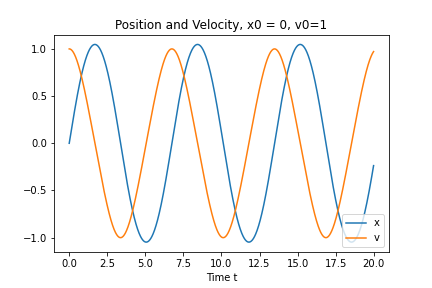
\includegraphics[scale=0.5]{4b_pos_vel.png}
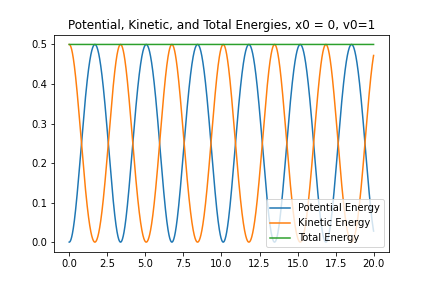
\includegraphics[scale=0.5]{4b_energy.png}
\item Now generate a trajectory with initial condition $x_0=0$ and $v_0=2.1$. Again make plots of position, velocity, kinetic, potential, and total energy as a function of time. These plots will look very different from the ones obtained before. Explain what is going on!\\
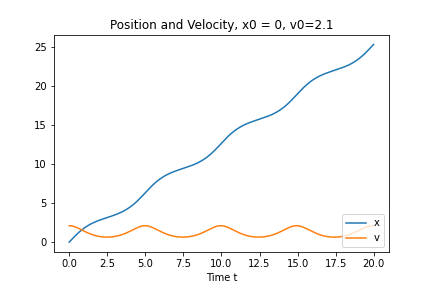
\includegraphics[scale=0.5]{4c_pos_vel}
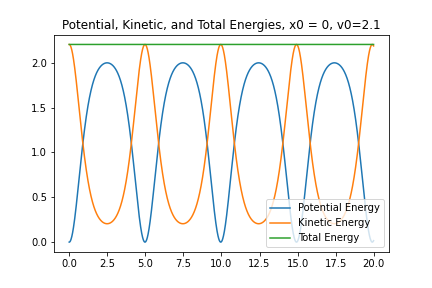
\includegraphics[scale=0.5]{4c_energy}
\soln{
I tried several starting velocities and saw that when $v_0 \geq 2$, the position function ceases to be periodic and increases with time. This happens because the maximum of our potential function ($U(x) = 1-cos(x)$) is 2. Because we still have kinetic energy when we reach the top of the potential, we move out of the first potential well. Instead of a swing, we get a perpetual roller-coaster}\\
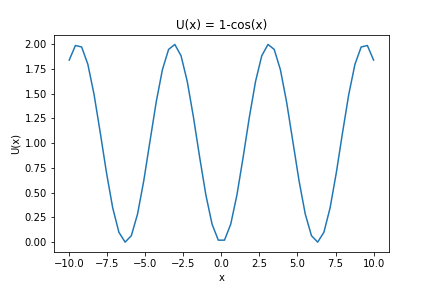
\includegraphics[scale=0.5]{4c_potential}
\end{enumerate}

\end{problemlist}  % enumeration of problems

%\begin{enumerate}[(a)~]
%\item
%\end{enumerate}

\end{document}
